\documentclass[]{beamer}

\usepackage{beamerthemesplit} 
\usepackage{movie15}
% Other themes include: beamerthemebars, beamerthemelined, 
%                       beamerthemetree, beamerthemetreebars  
\usepackage[utf8]{inputenc}
\inputencoding{utf8}
\usepackage[T2A]{fontenc}

\title[Speech and text alignment]{Analysis of knowledge requirements for speech and text alignment problem}
\author{Bartosz Kalińczuk}
\date{\today}

\begin{document}

\begin{frame}
  \titlepage
\end{frame}
\note{Talk for 15 minutes}

\section[Outline]{}

\begin{frame}
  \tableofcontents[hideallsubsections]
\end{frame}


\section{Audio model based alignment with word granularity}
\subsection{Required input}
\begin{frame}
    \frametitle{Required input}
    \begin{itemize}
        \item prepared audio model -> any similar
        \item limited knowledge of graphemes to phonemes conversions
        \item knowledge about alphabet and punctuation marks
    \end{itemize}
\end{frame}
\subsection{Outline of algorithm}
\begin{frame}
    \begin{itemize}
        \item Graphemes to phonemes conversion
        \item Converting text to HMM
        \item Viterbi algorithm
    \end{itemize}
\end{frame}
\subsection{Results - English audio model}
\begin{frame}
    \frametitle{English audio model}
    \begin{itemize}
        \item "Doktor Piotr" \newline
        After \textbf{38} seconds and after \textbf{62} words it incorrectly assigned 3 seconds to word “części” and it never recovered.
        \item  “Boże Narodzenie” \newline
        It has gone wrong after \textbf{257} seconds and \textbf{503} words on word “czarownicach”.
    \end{itemize}
\end{frame}

\begin{frame}
    \frametitle{English audio model}
    The statistics for “Boże Narodzenie” however shows, that before it goes bad it actually aligns first \textbf{503} words quite nicely:
    \begin{itemize}
        \item Maximum difference (start or end): 			\textbf{0.559s}
        \item Maximum difference (start or end), if label was to short at one end: 			\textbf{0.559s}
        \item Average difference  (start or end):			\textbf{0.032s}
    \end{itemize}
\end{frame}
\begin{frame}
    \frametitle{English audio model}
    Error counts depending on time thresholds:
    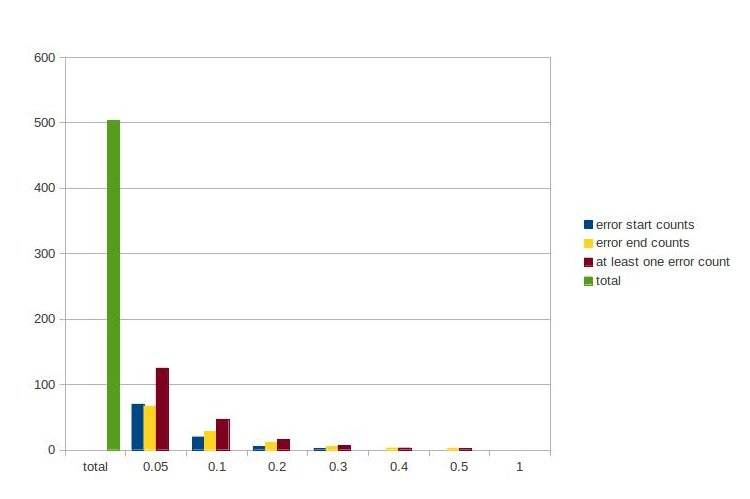
\includegraphics[scale=0.33]{boze_narodzenie_word_english_results.jpg}
\end{frame}
\subsection{Results - Russian audio model}
\begin{frame}
    \frametitle{Russian audio model - “Boże Narodzenie” statistics}
    \begin{itemize}
        \item Total number of words:				\textbf{1779}
        \item Maximum difference (start or end): 			\textbf{2.451s}
        \item Maximum difference (start or end), if label was to short at one end: 			\textbf{0.543s}
        \item Average difference  (start or end):			\textbf{0.016s}
    \end{itemize}
\end{frame}
\begin{frame}
    \frametitle{Russian audio model - “Boże Narodzenie” error counts}
    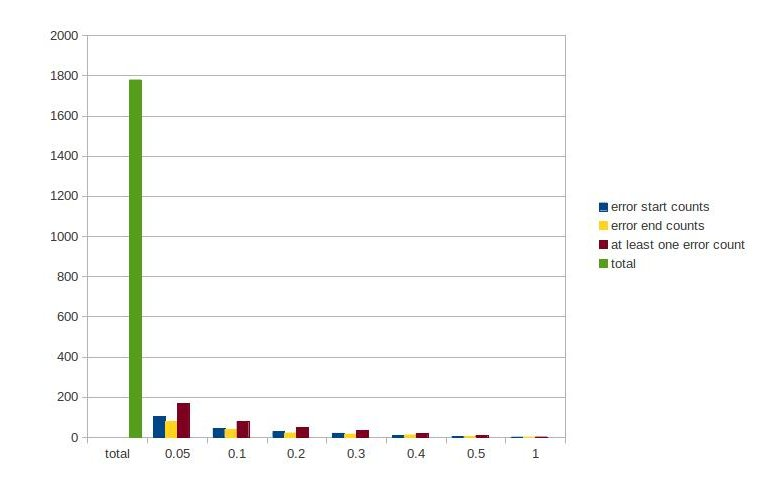
\includegraphics[scale=0.37]{boze_narodzenie_word_russian_results.jpg}
\end{frame}
\begin{frame}
    \frametitle{Russian audio model - “Doktor Piotr” sample statistics}
    \begin{itemize}
        \item Total number of words				\textbf{585}
        \item Maximum difference (start or end): 			\textbf{1.354s}
        \item Maximum difference (start or end), if label was to short at one end: 			\textbf{0.534s}
        \item Average difference  (start or end):			\textbf{0.033s}
    \end{itemize}
\end{frame}
\begin{frame}
    \frametitle{Russian audio model - “Doktor Piotr” sample error counts}
    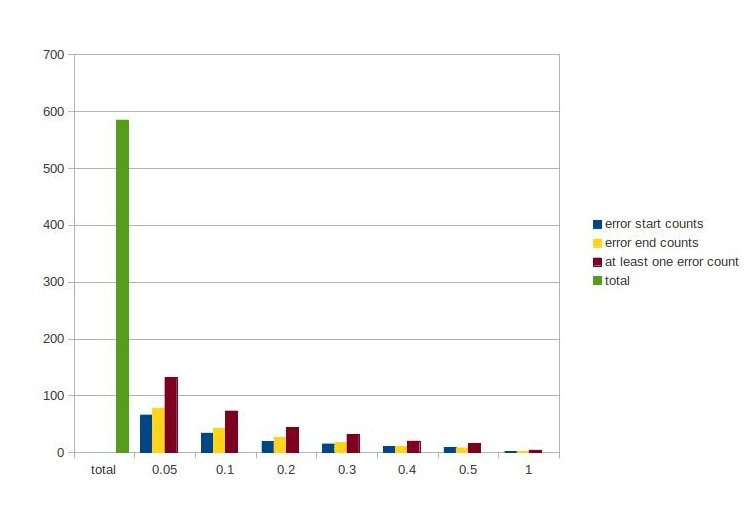
\includegraphics[scale=0.37]{doktor_piotr_word_russian_results.jpg}
\end{frame}

\section{Phoneme alignment}
\begin{frame}
\end{frame}
\subsection{Using sphinx loaded HMMs}
\begin{frame}
\end{frame}
\subsection{Using trained and simplified audio model}
\begin{frame}
\end{frame}
\subsection{Results - using Russian audio model}
\begin{frame}
    \frametitle{Testing sample}
    Tests are performed using Corpora corpus, which contains audio recordings of digits, names and some unusual sentences for tens of different speakers, and all of these recordings are tagged with phonemes. \newline
    Merged recording contains a 7 minutes and 26 second of audio data, a total of \textbf{843} spoken words and \textbf{3611} phoneme labels. \newline 
\end{frame}
\begin{frame}
    \frametitle{Statistics of phoneme alignment with Russian audio model}
    The test was 
    A resulting match contained \textbf{3570} of pairs.
    \begin{itemize}
        \item Average start difference: \textbf{ 0.0571s}
        \item Average end difference: \textbf{0.0574s}
        \item Maximum time difference:\textbf{0.516s}
    \end{itemize}
\end{frame}
\begin{frame}
    \frametitle{Error counts using Russian audio model}
    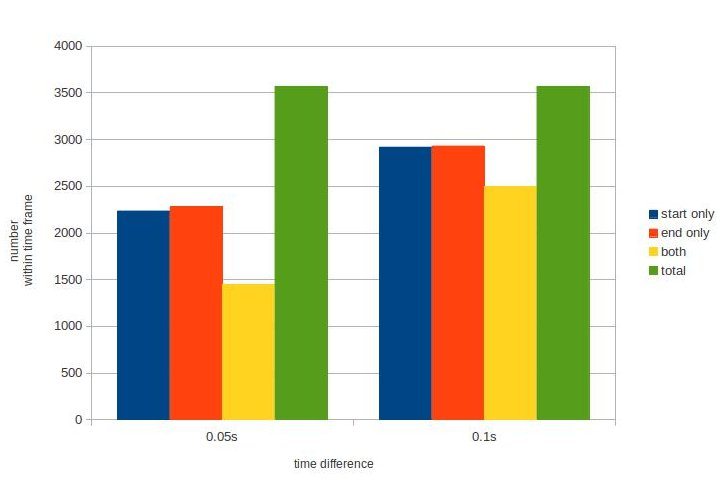
\includegraphics[scale=0.37]{corpora_phoneme_russian_counts.jpg}
\end{frame}
\begin{frame}
    \frametitle{Error counts (percentage) using Russian audio model}
    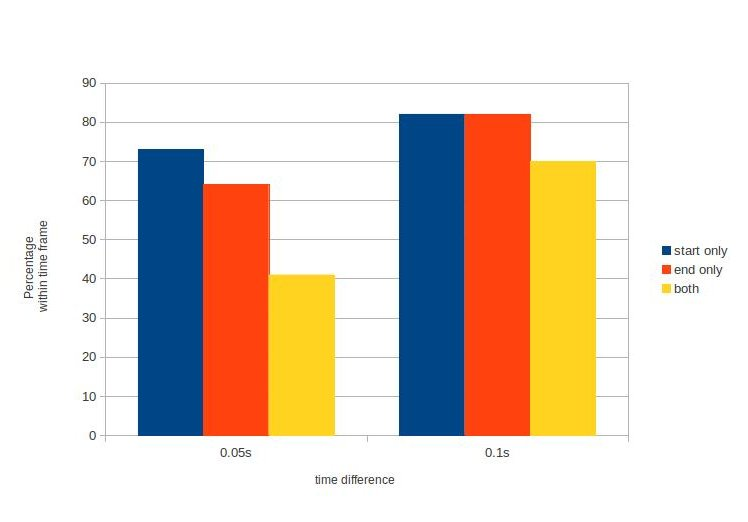
\includegraphics[scale=0.37]{corpora_phoneme_russian_results.jpg}
\end{frame}
\subsection{Results - using trained audio model}
\begin{frame}
    Matched phonemes contained \textbf{3611} pairs.
    \begin{itemize}
        \item Average start difference: \textbf{0.02402s}
        \item Average end difference: \textbf{0.02439s}
        \item Maximum time difference:\textbf{0.5131s}
    \end{itemize}
\end{frame}
\begin{frame}
    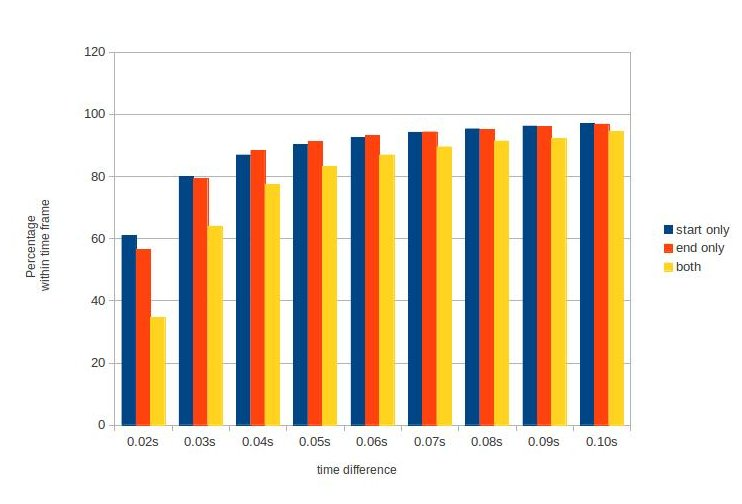
\includegraphics[scale=0.37]{corpora_phoneme_trained_results.jpg}
\end{frame}
\begin{frame}
    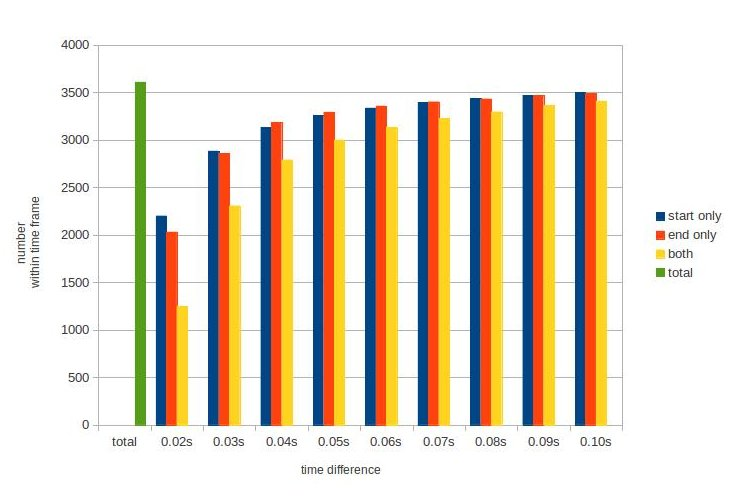
\includegraphics[scale=0.37]{corpora_phoneme_trained_counts.jpg}
\end{frame}

\section{Limited knowledge alignment}
\subsection{Pause/length based alignment}
\begin{frame}
\end{frame}
\subsection{Training audio model from large chunks}
\begin{frame}
\end{frame}
\subsection{Word recognition algorithm}
\begin{frame}
\end{frame}
\subsection{Results - sample of “Doktor Piotr”}
\begin{frame}
    \frametitle{Statistics - sample of “Doktor Piotr”}
    \begin{itemize}
        \item Total number of words				\textbf{585}
        \item Maximum difference (start or end): 			\textbf{0.422s}
        \item Maximum difference (start or end), if label was to short at one end: 			\textbf{0.371s}
        \item Average difference  (start or end):			\textbf{0.044s}
    \end{itemize}
\end{frame}
\begin{frame}
    \frametitle{Error counts - sample of “Doktor Piotr”}
    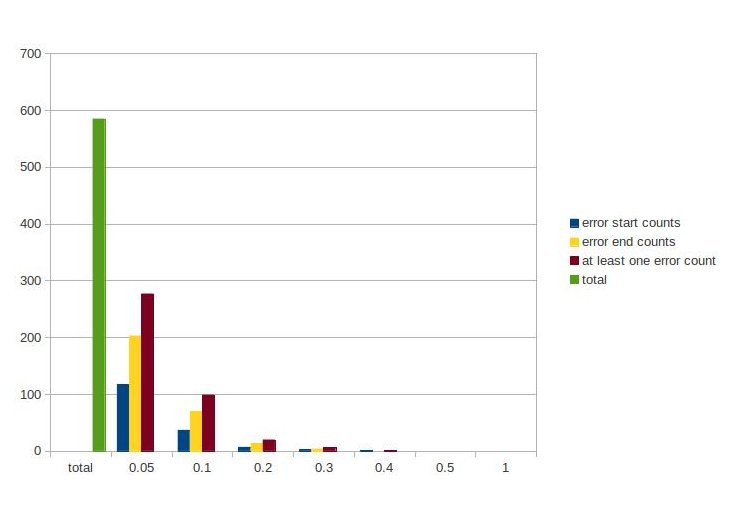
\includegraphics[scale=0.37]{doktor_piotr_length_based_counts.jpg}
    Dropping to 0 at 0.5 second difference, while getting to 99\% of correct tags for error of 300ms.
\end{frame}

\subsection{Results - “Boże Narodzenie”}
\begin{frame}
    \frametitle{Statistics - “Boże Narodzenie”}
    \begin{itemize}
        \item Total number of words				\textbf{1779}
        \item Maximum difference (start or end): 			\textbf{0.606s}
        \item Maximum difference (start or end), if label was to short at one end: 			\textbf{0.605s}
        \item Average difference  (start or end):			\textbf{0.046s}
    \end{itemize}
\end{frame}
\begin{frame}
    \frametitle{Error counts - “Boże Narodzenie”}
    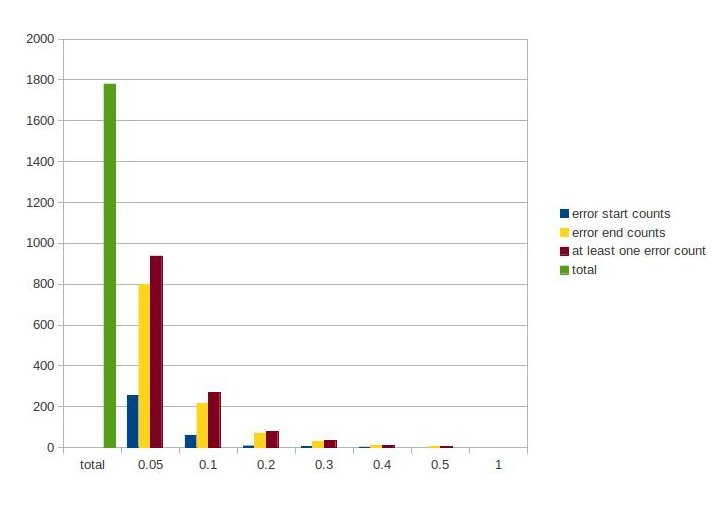
\includegraphics[scale=0.37]{boze_narodzenie_length_based_counts.jpg}
    Dropping to 0 at 1 second difference, while exceeding 98\% of correct tags for error of 300ms.
\end{frame}

\section{Synthesizer}
\subsection{Outline of algorithm}
\begin{frame}
\end{frame}
\subsection{Results}
\begin{frame}
    \frametitle{Sample synthesized texts}
    \begin{itemize}
        \item<1-> "W czasie suszy szosa sucha"
        \item<2-> "Za górami za lasami znajduję się wysoka wieża strzeżona przez smoka"
        \item<3-> "Litwo Ojczyzno moja ty jesteś jak zdrowie Ile cię trzeba cenić ten tylko się dowie Kto cię stracił Dziś piękność twą w całej ozdobie Widzę i opisuję bo tęsknię po tobie"
        \item<4-> "Chrząszcz brzmi w trzcinie w Szczebrzeszynie W szczękach chrząszcza trzeszczy miąższ Czcza szczypawka czka w Szczecinie"
        \item<5-> "Rosja przedwojenna była wymarzoną areną dorobku dla ludzi tego typu zwłaszcza pochodzących z Królestwa"
    \end{itemize}
\end{frame}

\section{Conclusions}
\begin{frame}
    \frametitle{Conclusions}
\end{frame}
\begin{frame}
    \frametitle{Future works}
\end{frame}

%\subsection{Simple slide with three points shown in succession}
%
%\begin{frame}
%  \frametitle{Simple slide with three points shown in succession}   % Insert frame title between curly braces
%
%  \begin{itemize}
%  \item<1-> Point 1 (Click ``Next Page'' to see Point 2) % Use Next Page to go to Point 2
%  \item<2-> Point 2  % Use Next Page to go to Point 3
%  \item<3->
%  \end{itemize}
%\end{frame}
%\note{Speak clearly}  % Add notes to yourself that will be displayed when
%                      % typeset with the notes or notesonly class options
%
%
%\section{Slide with two columns: items and a graphic}
%
%\begin{frame}
%  \frametitle{Slide with two columns: items and a graphic}   % Insert frame title between curly braces
%  \begin{columns}[c]
%  \column{2in}  % slides are 3in high by 5in wide
%  \begin{itemize}
%  \item<1-> First item
%  \item<2-> Second item
%  \item<3-> ...
%  \end{itemize}
%  \column{2in}
%  \framebox{Insert graphic here % e.g. \includegraphics[height=2.65in]{graphic}
%  }
%  \end{columns}
%\end{frame}
%\note{The end}       % Add notes to yourself that will be displayed when
%		     % typeset with the notes or notesonly class options

\end{document}

